\documentclass[14pt, a4paper, oneside]{extarticle}
\usepackage[T2A]{fontenc}
\usepackage[utf8]{inputenc}
\usepackage[russian]{babel}
\usepackage{hyperref}
\usepackage{xcolor}
\usepackage{geometry}
\geometry{top=1cm, bottom=0.5cm, left=1cm, right=1cm}
\usepackage{graphicx}
\usepackage{float}
\usepackage{wrapfig}
\usepackage{fontawesome5}
\usepackage{ragged2e}
\usepackage{microtype}

\hypersetup{
    colorlinks=false,
    allcolors=blue,
    pdfborderstyle={/S/U/W 0.5},
    allbordercolors=blue
}

\begin{document}

% Фото

%\begin{wrapfigure}{l}{0.18\textwidth}
%	\vspace{\intextsep}
%    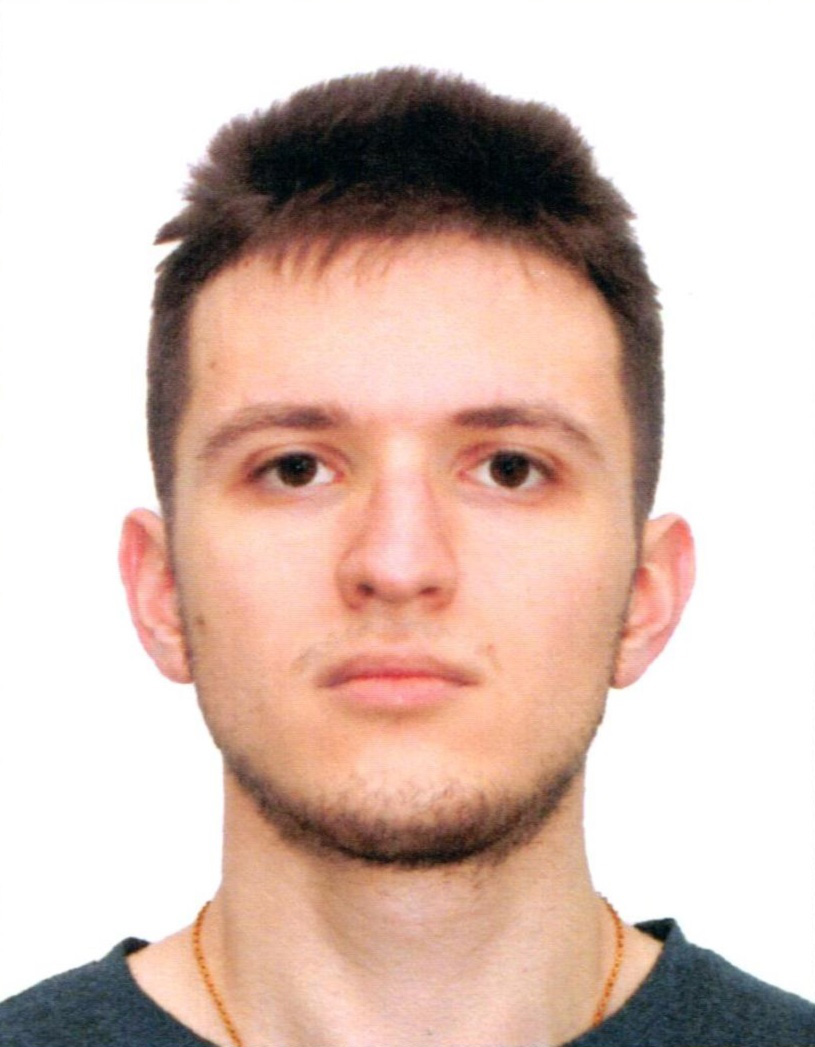
\includegraphics[width=0.18\textwidth]{personal_photo.jpg}
%\end{wrapfigure}

% Заголовок

\begin{center}
    \textbf{\LARGE Куценко Максим Дмитриевич}
    
    \textit{\Large Системный аналитик}
\end{center}

\begin{center}
	\vspace{-0.5\intextsep}
	\small
    \faPhone* \space +7 (985) 647-53-50 | \faEnvelope \space \url{maximkuts23@gmail.com} | \faGithub \space \url{github.com/Crazy5202} | \faTelegram \space \href{t.me/Crazy523}{@Crazy523}
\end{center}

% Подзаголовок Образование

\begin{flushleft}
	\vspace{-\intextsep}
	\large Образование
\end{flushleft}

\vspace{-0.8\intextsep}
\hrule

% Магистратура

\begin{flushleft}
	\vspace{-0.8\intextsep}
	\quad
	\textbf{Московский авиационный институт}
	\hfill
	Москва
\end{flushleft}

\begin{flushleft}
	\vspace{-\intextsep}
	\quad
	\textit{\footnotesize Магистр, %фундаментальная информатика и информационные технологии} 
	искусственный интеллект и суперкомпьютерное моделирование}
	\hfill
	\textit{\small Авг. 2026 - н.в.}
\end{flushleft}

% ДПП по системной аналитике

\begin{flushleft}
	\vspace{-0.8\intextsep}
	\quad
	\textbf{Московский авиационный институт, Т1}
	\hfill
	Москва
\end{flushleft}

\begin{flushleft}
	\vspace{-\intextsep}
	\quad
	\href{https://github.com/Crazy5202/job_application_form/tree/main/portfolio/T1}{\textit{ДПП, системный аналитик}}
	\hfill
	\textit{\small Фев. 2025 - Июнь 2025}
\end{flushleft}

% Бакалавриат

\begin{flushleft}
	\vspace{-0.8\intextsep}
	\quad
	\textbf{Московский авиационный институт}
	\hfill
	Москва
\end{flushleft}

\begin{flushleft}
	\vspace{-\intextsep}
	\quad
	\textit{Бакалавр, прикладная математика и информатика}
	\hfill
	\textit{\small Авг. 2022 - Авг. 2026}
\end{flushleft}

%\begin{flushleft}
%	\vspace{-1.2\intextsep}
%	\quad
%	\textit{\small суперкомпьютерное моделирование}
%\end{flushleft}

% Подзаголовок Практический опыт

\begin{flushleft}
	\vspace{-\intextsep}
	\large Практический опыт
\end{flushleft}

\vspace{-0.8\intextsep}
\hrule

% K2

\begin{flushleft}
	\vspace{-0.8\intextsep}
	\quad
	\href{https://github.com/Crazy5202/job_application_form/tree/main/portfolio/K2}{\textbf{Технический трек AI Boostcamp}}
	\hfill
	Москва
\end{flushleft}

\begin{flushleft}
	\vspace{-1\intextsep}
	\quad
	\textit{К2 Нейротех}
	\hfill
	\textit{\small Нояб. 2025 - Дек. 2025}
\end{flushleft}

% Список K2

\begin{itemize}
	\vspace{-2\intextsep}
	\item Построение архитектуры (C4) и жизненного цикла (DFD) RAG-системы
	\vspace{-0.8\intextsep}
    \item Проектирование пайплайнов обработки данных и интеграция LLM (n8n)
\end{itemize}

% eComm

\begin{flushleft}
	\vspace{-\intextsep}
	\quad
	\href{https://github.com/Crazy5202/job_application_form/blob/main/portfolio/eComm_C4.pdf}{\textbf{Бэкенд интернет-магазина (учебный проект)}}
	\hfill
	Москва
\end{flushleft}

\begin{flushleft}
	\vspace{-1\intextsep}
	\quad
	\textit{Московский авиационный институт}
	\hfill
	\textit{\small Фев. 2025 - Июнь 2025}
\end{flushleft}

% Список eComm

\begin{itemize}
	\vspace{-2\intextsep}
	\item Проектирование микросервисной архитектуры решения (C4)
	\vspace{-0.8\intextsep}
	\item Проектирование схемы БД и миграций (SQLAlchemy, Alembic)
	\vspace{-0.8\intextsep}
	\item Разработка спецификаций REST API для микросервисов на FastAPI
	\vspace{-0.8\intextsep}
	\item Построение ролевой модели доступа (RBAC) на основе куки
	\vspace{-0.8\intextsep}
	\item Конфигурация доступа к сервисам через reverse proxy (Traefik)
	\vspace{-0.8\intextsep}
	\item Тестирование контрактных взаимодействий (Postman)
	\vspace{-0.8\intextsep}
    \item Руководство командой (4 человека), ведение 

    \vspace{-0.5\intextsep}
    бэклога и проектной документации  (ТЗ, диаграммы UML) 
\end{itemize}

% Кинотеатр

\begin{flushleft}
	\vspace{-\intextsep}
	\quad
	\textbf{Онлайн-кинотеатр (учебный проект)}
	\hfill
	Москва
\end{flushleft}

\begin{flushleft}
	\vspace{-1\intextsep}
	\quad
	\textit{Московский авиационный институт}
	\hfill
	\textit{\small Сент. 2024 - Дек. 2024}
\end{flushleft}

% Список Кинотеатр

\begin{itemize}
	%\vspace{-0.8\intextsep}
	%\item Парсинг постеров фильмов с IMDB и загрузка в S3-хранилище
	\vspace{-2\intextsep}
	\item Проектирование сервисной архитектуры решения (C4)
	\vspace{-0.8\intextsep}
	\item Разработка спецификаций REST API для Backend и ML сервисов
	\vspace{-0.8\intextsep}
    \item Тестирование контрактных взаимодействий (Postman)
	\vspace{-0.8\intextsep}
    \item Руководство командой (4 человека), ведение 

    \vspace{-0.5\intextsep}
    бэклога и проектной документации  (ТЗ, диаграммы UML)
\end{itemize}

% ЭДО

\begin{flushleft}
	\vspace{-0.8\intextsep}
	\quad
	\href{https://github.com/Crazy5202/job_application_form/tree/main/portfolio/EDMS}{\textbf{\smallСервис распознавания подписей и печатей в документах (учебный проект)}}
	\hfill
	Москва
\end{flushleft}

\begin{flushleft}
	\vspace{-1\intextsep}
	\quad
	\textit{Московский авиационный институт, МТС}
	\hfill
	\textit{\small Фев. 2024 - Июнь 2024}
\end{flushleft}

% Список ЭДО

\begin{itemize}
	\vspace{-2\intextsep}
    \item Сбор и формализация бизнес-требований от партнёра проекта
    \vspace{-0.8\intextsep}
    \item Проектирование монолитной архитектуры решения (C4)
	\vspace{-0.8\intextsep}
    \item Руководство командой (9 человек), ведение 
    
    \vspace{-0.5\intextsep}
    бэклога и проектной документации  (ТЗ, диаграммы UML)
    \vspace{-0.8\intextsep}
    \item Результат представлен на форуме электронного документооборота,
    
    \vspace{-0.5\intextsep}
    получил положительные оценки
   	\vspace{-0.8\intextsep}
    \item Рекомендован к внедрению на основе отзыва партнёра проекта
    \vspace{-0.8\intextsep}
    \item Занял 1 место в конкурсе работ на потоке
\end{itemize}

% Новая страница
\pagebreak

% Подзаголовок Технологический стек

\begin{flushleft}
	\vspace{-\intextsep}
	\large Технологический стек
\end{flushleft}

\vspace{-0.8\intextsep}
\hrule

% Скиллы

\vspace{0.5\intextsep}

\textbf{Моделирование архитектуры и процессов:} C4, UML, BPMN, DFD, ERD

\textbf{Проектирование API и форматы данных:} Swagger, JSON, XML

\textbf{Наблюдаемость:} Grafana, Prometheus, Loki, Promtail, Logstash, Kibana

\textbf{Очереди сообщений:} Kafka, RabbitMQ

\textbf{Базы данных:} PostgreSQL, MongoDB, Redis, Elasticsearch, ClickHouse

\textbf{Языки программирования:}  SQL, Python

\textbf{Инфраструктура и интеграции:} Linux, Git, Docker, Traefik, n8n

\textbf{Методологии и управление:} Agile, Scrum, Jira, Trello, Confluence, Excel

\textbf{Иностранные языки:} Английский C1

% Подзаголовок О себе

\begin{flushleft}
	\vspace{-\intextsep}
	\large О себе
\end{flushleft}

\vspace{-0.8\intextsep}
\hrule

% О себе
\begin{sloppypar}
	\vspace{0.8\intextsep}
	\quad
	Начинающий системный аналитик с опытом проектирования асинхронной микросервисной архитектуры (очереди сообщений, балансировка нагрузки) и управления командой разработки (до 10 человек). Умею переводить бизнес-требования в технические спецификации и выстраивать эффективную коммуникацию между заказчиком и разработчиками. Технический бэкграунд даёт мне глубокое понимание жизненного цикла ПО. Интересуюсь системной инженерией, архитектурой и когнитивной психологией.
	\justify
\end{sloppypar}

\end{document}